\chapter{Discussion}\label{ch:disc}

\section{BNIG model limitations}

\subsection{State Independent Variance}

One constraint of the BNIG model is that it assumes a constant variance over all states given an action. This does not necessarily deteriorate performance as much as one might expect. \cite{azziz_2018} achieves performance better than DQN in multiple ALE games with the same restriction. However it seems that this might be a problem on environments that require more complex exploration. For example Montezuma's revenge is not included in the attempts in \cite{azziz_2018} and attempts at using the BNIG model quickly converged to a zero variance and zero reward reward policy.

It is likely that an environment such as Montezuma's Revenge requires the variance to be adjusted per state. In these environments the same action might lead to states with largely different variances based on the current state. Consider a left action on the edge of one room in Montezuma's Revenge. This leads to a new room with a large set of possibilities and thus should have a large variance. In another case a left action might cause the character to fall to its death. The agent should recognize what is happening and have a low variance estimate that it won't receive anymore reward. With the current BNIG model the variance estimate for the left action will have to be between the two resulting in too much exploration in states the model should be certain about and more importantly too little exploration in unexplored states.

\begin{figure}[H]
    \centering
    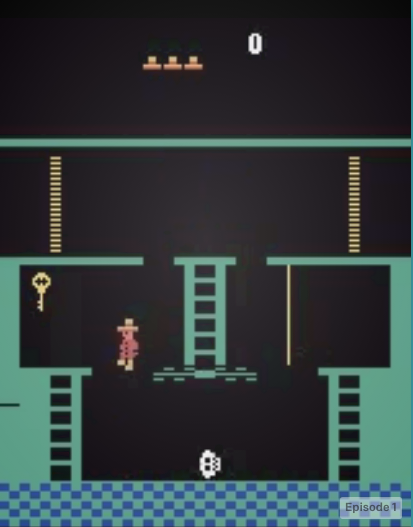
\includegraphics[scale=0.25]{montezuma.png}
    \captionsetup{width=.7\linewidth}

    \caption{\textbf{Montezuma's Revenge}: An left moving agent falling to its death should have a low variance estimate of future reward compared to a left moving agent switching room.}
\end{figure}

In a game like cartpole this is still the case but to much smaller extent. The state of the cartpole has little effect on the variance of the next state. Once a policy is learned the pole is relatively certainly going to stay balanced over future states meaning low variance. If the pole is starting to fall the pole will most likely completely fall leading to termination, once again with low variance. In these types of environments one should expect BNIG to perform well.

\subsection{Variance Stability}

Another shortcoming of the BNIG DQN method is the instability of the variance estimate. Though an increase in the prior scale parameter improves performance this lowers variance based on a hyperparameter rather than the data. It greatly constricts the exploration and must be tuned on an environment to environment basis. Further developments should focus on how to stabilize this variance to allow for weaker priors. There are multiple issues that could decrease the stability of the variance.


\subsubsection{Maximization Bias}

One source of instability could be maximization bias\citep[p.~134]{sutton_barto_2018} occurring on the variance estimate. Early in the learning process the maximum operator on the target leads to picking actions that lead to high variance states as these provide the highest values. This leads to higher variance targets which starts a feedback loop that can lead to the large jumps in the rate parameter of the inverse gamma distribution as seen in figure \ref{fig:scale_stability}.

A solution to the maximization bias in regular Q-learning is double Q-learning as discussed in chapter \ref{ch:theo}. This consists of creating two completely decoupled models and for each update use one for target action selection and one for action-value calculation. This doubles the memory complexity of the model but keeps the same computational complexity. The double DQN uses an approximation to this by using the target network for target action selection and the online network for action-value calculation. This is also what is done with the BNIG target model in this thesis. However a complete decoupling by creating two BNIG models per action might help reduce the variance instability with a relatively small memory cost.

\subsubsection{State Independent Variance}

It has already been discussed how the state independent variance might be constraining the environments BNIG is useful on. However it is also possible that this is leading to variance instability on all environments. 

Consider regular Q-learning. The magnitude of the Q-values is controlled by the terminal states where the target is bound by the maximum reward from the environment. As Q-learning learns, this bounded value is propagated backwards towards the initial state, leading to Q-values that are realistic relative to the return from the environment.

In the variance case one should expect the same behavior. The propagation tests in chapter \ref{ch:linear} showed that given a known posterior state all other states leading up to this will converge towards the same variance. However this test is in a tabular setting where each state has its own variance parameter. In the linear setting a state that should have low variance, such as a penultimate state, will have to have a similar variance to all other states. As such there is no low variance state that slowly bounds the variance of all states. This allows for an ever increasing variance. If one instead has a state dependent variance one could expect a similar result as in Q-learning, with the low variance terminal states slowly bounding the variance of the rest of the states.

\section{Results on Corridor Environment}

\subsection{Linear versus Neural network}

One surprising result was the difference in performance on the corridor environment between the linear and neural network BNIG method. In the linear case it was shown that the per episode BNIG model outperformed the $\varepsilon$-greedy method. In the neural network setting the it was the opposite case with the $\varepsilon$-greedy DQN outperforming the BNIG DQN. Part of this can be explained by the extra stochasticity introduced through gradient descent over a larger number of parameters leading to more exploration regardless of the method used \citep{carlos_2018}. 

However this does not explain why the BNIG DQN performs worse than the linear BNIG on the same problem. In addition there was no observed instability over the noise variance, hence no improvement on the prior tuned BNIG DQN.

In hindsight one possible reason for the worse performance is that the linear corridor setup is biased towards the BNIG model. The input state in the linear corridor environment, as seen in the implementation details in \ref{a:lin_corridor}, is a vector of the number of steps taken and the current state. As such the requirement for the BNIG model to reach the end of the corridor is that the two coefficients for the right action are sampled large enough for the sum to be larger than action 0 in all states. The $\varepsilon$-greedy method on the other hand needs to randomly move to the right for every state, giving a probability $\varepsilon^N$ of reaching the end of the corridor based on the exploration policy. In the neural network case the BNIG model has an input size of 20 making it substantially less probable to reach the final state.

\subsection{Network Stability}

Another interesting observation during training was that the BNIG DQN does in fact reach the terminal state multiple times each iteration. In addition increasing the shape parameter improved performance despite this leading to decrease exploration. This indicates that the disappointing results of the BNIG DQN on the corridor environment is not due to too low exploration. 

This introduces another possible short coming of the method, the possibility that the underlying network is unstable and this in turn results in an unstable BNIG. At first sight the neural network stability might seem independent of the parameter variance since it trains on the MAP estimates. However a large variance parameter allows for large shifts in the MAP estimate. It is therefore possible that the high shape parameter simply stabilizes the neural network leading to more stable variance estimates and thus better performance. This is a chicken and the egg problem and further research would be required to find what part to focus stabalization efforts on.

\section{Method Improvements}

\subsection{Allowing for State Dependent Variance}

A few attempts were made to make the variance state dependent. Due to computational and time constraints these are not included in this thesis. However this subsection highlight some of the possible methods for doing this and which are most promising.

One approach would be to use a random effects model\citep[p.~382-383]{gelman_2013} which allows different variance levels in different groups. The main challenge would then be how to group different state. This could either be done through manual feature engineer or some unsupervised learning method. The first in undesirable in the general case as it requires manual work and subjective modeling of the environment, reducing the generalizability of the model. The latter would require further research.

To avoid this one could instead set up a new model that incorporates the unequal variances and correlated errors by considering $y \sim N(X\beta, \Sigma_y)$ instead of $y \sim N(X\beta, \sigma_a)$.  However these models are more complicated to setup and usually some prior knowledge about the structure of the covariance matrix. It could be possible to somehow incorporate the RL structure to define a weighting for bayesian weighted regression\citep[p.~370-373]{gelman_2013}. 

One way to define this weighting structure would be to use a model that assumes a known noise variance per datapoint. This is equivalent to a diagonal $\Sigma_y$. Then one could try to directly model the variance parameters by considering the structure of the RL problem. This approach is similar to the one introduced in \cite{donoghue_2017}. However note that the resulting model would be substantially different as instead of propagating explicitly through the uncertainty bellman equation the propagation would occur through sampling the target values.

\subsection{Exponential Forgetting}

Exponential forgetting was used as a quick solution to the non-stationary target issue due to it's simple implementation and low computational cost. However it does not have a strong statistical base and makes it impossible to use stronger priors without leading to large differences in agent behavior. There exists plenty of literature in statistics on more informed filtering to handle non-stationary targets. One could for example build a state space model to perform this filtering. The main difficulty is finding a method the balances the accuracy of the filter with the computational cost of running the filter.

\subsection{Runtime}

The runtime of the BNIG DQN model is worse than the DQN model. On acrobot the DQN model averaged 220 frames per second during training while the BNIG DQN model averaged 145. However the BNIG implementation has not been optimized. Notably the covariance posterior update can be reduced from $O(p^3)$ to $O(p^2)$ where $p$ is the size of the final layer by using the Sherman-Morrison-Woodbury formula as in \cite{donoghue_2017}. 

\subsection{Separate N-Step}

A minor improvement would be to allow separate $n$-step updates for the neural network and the BNIG model. As seen in chapter \ref{ch:linear} increasing the $n$ can lead to much better variance propagation and better results in the RL setting. However a high $n$-step reduces performance and earlier papers have found $n=3$ performs best on ALE\citep{hessel_2017}. However since the training procedures for the BNIG model and network are separate one can use separate $n$ values for each model. This is used in \cite{donoghue_2017} where n is set to 150 for only the variance model.

\cleardoublepage